\subsection{Types of heat source}
\begin{itemize}
	\item Point source\\
	The type of heat source resembles a tiny object produce thermal conduction inside the domain. The point source locates at a fixed coordinate $(x_0,y_0)$ and thermal conduction capacity $h(t)$. These component form the right hand side of heat equation
	$$
	F(x,y,t) = \delta_{x_0 y_0}(x,y)\times h(t)
	$$
	Where $\delta_{x_0 y_0}$ is the dirac delta function use for locating the heat point source. For instance, the dirac delta function can be like:
	$$
	\delta_{x_0 y_0} = \dfrac{n}{\cosh(n(x-x_0))^2}\times\dfrac{n}{\cosh(n(y-y_0))^2}
	$$
	\begin{figure}[ht]
		\centering
		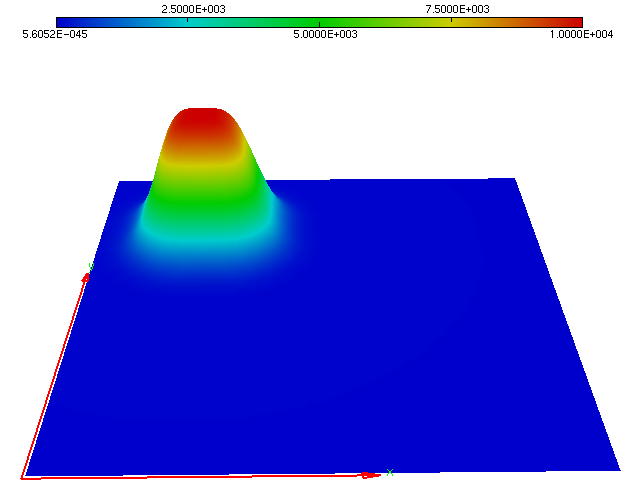
\includegraphics[width=4cm]{figures/dirac}
		\caption{Illustration of chosen dirac delta function.}
	\end{figure}
	\item Wall source: Assuming the heat source attaches to a part of domain wall. Thermal conduction provide by that heat source can be express by various way.\\
	The fixed temperature walls is the most basic way to resemble a heat source. This type of wall is respective with the Diriclet boundary condition.\\
	The other type of wall source provide the heat flux through the wall, respective with Neumann boundary condition.\\
\end{itemize}